\section{Producción}

En esta fase se llevaron a cabo las pruebas de carga donde se simulará la interacción de los usuarios con la aplicación para validar el rendimiento de la aplicación cuando la aplicación está disponible para su uso.

 Para tal efecto se probaron 3 \emph{endpoints} o URIs del API. Que se escogieron por considerarse que son las que serán altamente usadas y posiblemente las más críticas, se las puede ver en la tabla \ref{tab:tests_rendimiento}.

 % \begin{enumerate}
 %   \item Obtener la lista de Lugares,
 %   \item Obtener el \emph{Nodo} (del mapa de rutas) más cercano a la posición del Usuario o del Lugar.
 %   \item Obtener la ruta óptima entre 2 \emph{Nodos}.
 % \end{enumerate}

 \begin{table}[H]
   \begin{center}
     \begin{tabularx}{0.9\textwidth}{ c X  X }
       \toprule
       \textbf{C\'odigo} &
         \multicolumn{1}{c}{\textbf{Objetivo}} &
         \multicolumn{1}{c}{\textbf{Endpoint}} \\

\midrule
PR01 &
Obtener la lista de Lugares.
&
GET \url{api/v1/places/} \\

 \addlinespace
 PR02 &
 Obtener el \emph{Nodo} (del mapa de rutas) más cercano a la posición (latitud y longitud) del Usuario o del Lugar.
 &
 GET \url{api/v1/ways/node/:lat/:lon} \\


  \addlinespace
  PR03 &
  Obtener la ruta óptima entre 2 \emph{Nodos}, el nodo origen (\emph{source}) y el nodo destino (\emph{target}) .
  &
  GET \url{api/v1/ways/route/:target} \tab \url{/:source} \\

       \bottomrule
     \end{tabularx}
     \caption{Pruebas de rendimiento}
     \label{tab:tests_rendimiento}
   \end{center}
 \end{table}


 Se consideró que la aplicacion deberia soportar por lo menos la interacción de 100 usuarios, por lo que se tomó esta cantidad como caso base y sobre la cual se aumentará a 500 usuarios y por último lugar, 1000 usuarios interactuando con la aplicación al mismo tiempo.

  Para llevar a cabo estas pruebas se hizo uso de \emph{JMeter} y a continuación se describirán los resultados encontrados.

  En la figura \ref{fig:jmeter_result}, se puede observar que los \emph{requests} de 100 usuarios hacia la aplicación tiene tiempos de retorno buenos, para la prueba PR02 y PR03 se obtuvo un promedio de 0.8 segundos en cambio para la prueba PR01 el tiempo de ejecución se incrementó hasta un promedio de 8 segundos pero en ninguna de las 3 pruebas se generó algún error de respuesta del servidor. En cambio cuando 500 usuarios interactúan con la aplicación se puede observar que \emph{obtener la lista de lugares} ya presenta errores y los tiempos de retorno aumentaron considerablemente, la misma tendencia se puede ver con la ejecución de 1000 usuarios.


  \begin{figure}[H]
        \begin{center}
          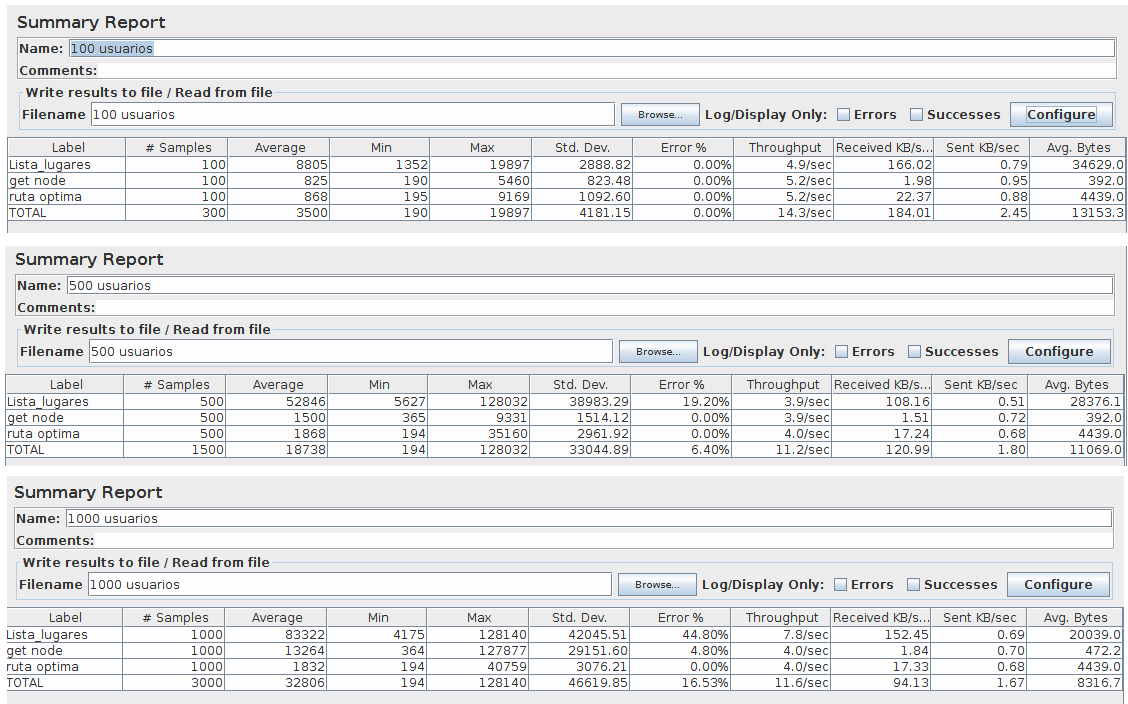
\includegraphics[width=0.9\textwidth]{jmeter_result}

          \caption{Resultados obtenidos de JMeter.}
          \label{fig:jmeter_result}
          \caption*{Fuente: Elaboración propia.}
        \end{center}
  \end{figure}

 En la figura \ref{fig:azure_report}, se puede ver el consumo de recursos por parte del servidor durante la ejecución de las pruebas de carga, se puede notar que a pesar de haber generado errores cuando la carga de usuarios es elevada, el servidor regresa a un estado estable.

  \begin{figure}[H]
        \begin{center}
          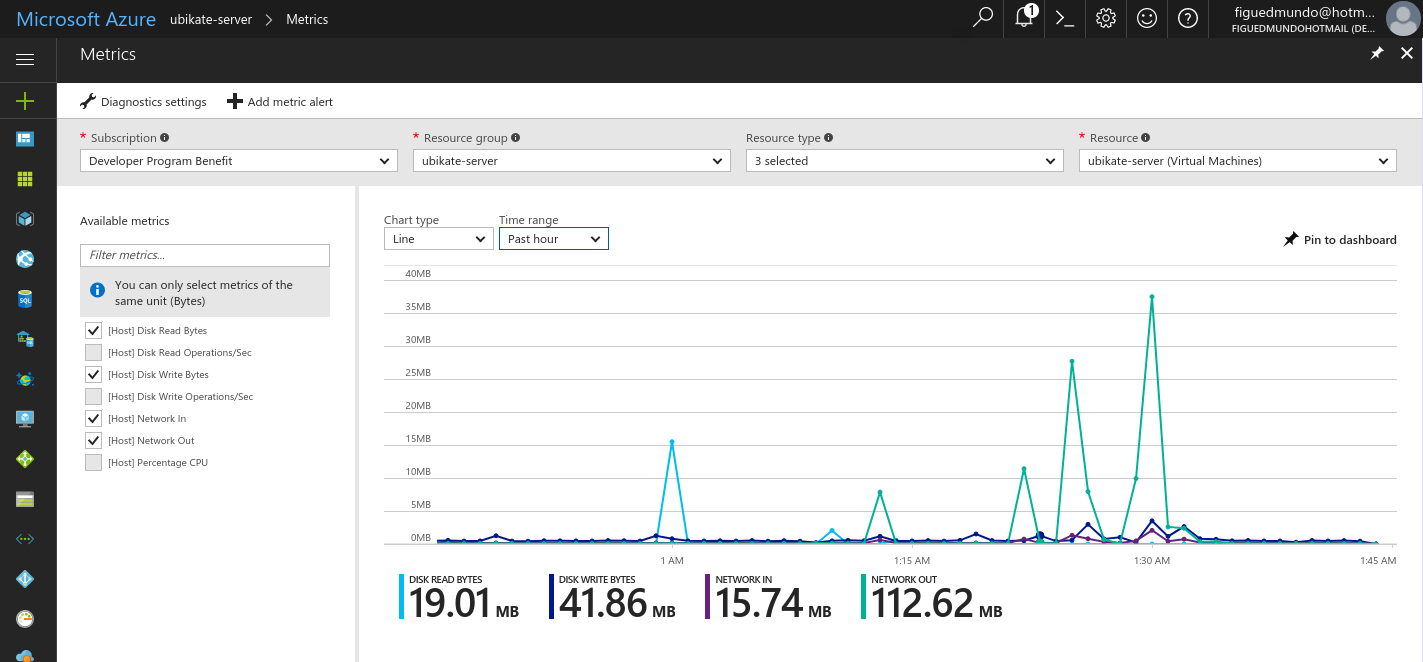
\includegraphics[width=0.85\textwidth]{azure_report}

          \caption{Reporte del servidor Azure.}
          \label{fig:azure_report}
          \caption*{Fuente: Elaboración propia.}
        \end{center}
  \end{figure}



  De la ejecución de las pruebas de carga se puede concluir que es necesario analizar y refactorizar los módulos encargados de \emph{obtener la lista de usuarios}, tarea que se puede realizar en una futura entrega del producto.

  Tomando en cuenta que para una carga de 100 usuarios se observaron tiempos de respuesta aceptables por el cliente, se considera que la aplicación cumple con los objetivos de rendimiento trazados.
